\documentclass[12pt]{article}

\usepackage{sbc-template}
\usepackage{graphicx,url}
\usepackage{float}
\usepackage[utf8]{inputenc}
\usepackage[brazil]{babel}
\usepackage[latin1]{inputenc}  

     
\sloppy

\title{Particle Swarm Optimization\\ Um estudo sobre o algoritmo PSO}

\author{César Eduardo de Souza\inst{1},\\ Guilherme Diel\inst{1}}


  \address{Departamento de Ciência da Computação \\ Universidade do Estado de Santa Catarina
  (UDESC) -- Joinville, SC -- Brazil
  \email{\{cesar.souza, guilherme.diel\}@edu.udesc.br}
}

\begin{document} 

\maketitle

     
\begin{resumo} 
  Algoritmos heurísticos são fundamentais para a busca de soluções satisfatórias em problemas complexos de otimização. Um dos métodos mais populares é o \textbf{Particle Swarm Optimization} (PSO), inspirado no comportamento coletivo de enxames naturais. Este algoritmo é capaz de resolver problemas NP-Hard e NP-Completo, como funções de benchmark em otimização contínua. Neste trabalho, apresentamos uma implementação do \textbf{PSO} para otimização das funções de Ackley e Griewank, analisando o desempenho do algoritmo em diferentes dimensões e discutindo possíveis aplicações futuras e comparações com outras abordagens.
\end{resumo}


\section{Introdução}
\label{sec:introducao}
% Contextualização do problema/tarefa e revisão da literatura.
A busca por soluções eficientes para problemas de otimização combinatória e contínua motivou o desenvolvimento de diversos algoritmos heurísticos e metaheurísticos. Entre eles, destaca-se o \textbf{Particle Swarm Optimization} (PSO), proposto por Kennedy e Eberhart em 1995, inspirado no comportamento social de pássaros e cardumes.

O PSO é amplamente utilizado para resolver problemas de otimização devido à sua simplicidade, facilidade de implementação e capacidade de convergência para soluções de alta qualidade. O algoritmo consiste em um conjunto de partículas (soluções candidatas) que exploram o espaço de busca, ajustando suas posições com base em suas experiências individuais e coletivas.

Neste trabalho, investigamos o desempenho do PSO na otimização das funções de Ackley e Griewank, que são funções de benchmark clássicas em otimização contínua. Avaliamos o comportamento do algoritmo em diferentes dimensões e discutimos os resultados obtidos.

Este relatório está organizado da seguinte maneira: a seção 2 apresenta a metodologia de desenvolvimento e a descrição do algoritmo PSO. Em seguida, na seção 3, são abordados os experimentos realizados e os resultados obtidos. A seção 4 discute a análise dos resultados e, por fim, a seção 5 apresenta as conclusões e sugestões para trabalhos futuros.

\section{Metodologia de Desenvolvimento}
\label{sec:metodologia_de_desenvolvimento}

O algoritmo \textbf{Particle Swarm Optimization} (PSO) funciona da seguinte forma:
\begin{enumerate}
  \item Inicializar uma população de partículas com posições e velocidades aleatórias no espaço de busca.
  \item Para cada partícula, avaliar a função objetivo na posição atual.
  \item Atualizar a melhor posição individual (\textit{pbest}) e a melhor posição global (\textit{gbest}).
  \item Atualizar a velocidade e a posição de cada partícula de acordo com as equações:
    \begin{equation}
      v_{i}(t+1) = w v_{i}(t) + c_1 r_1 (pbest_{i} - x_{i}(t)) + c_2 r_2 (gbest - x_{i}(t))
    \end{equation}
    \begin{equation}
      x_{i}(t+1) = x_{i}(t) + v_{i}(t+1)
    \end{equation}
    onde $w$ é o fator de inércia, $c_1$ e $c_2$ são os coeficientes cognitivo e social, e $r_1$, $r_2$ são números aleatórios em $[0,1]$.
  \item Repetir os passos 2 a 4 até atingir o critério de parada (número máximo de iterações ou tolerância).
\end{enumerate}

A implementação foi realizada em \textit{Python}, utilizando a biblioteca \textit{Numpy} para operações vetoriais e \textit{Matplotlib} para visualização dos resultados.

\begin{figure}[H]
    \centering
    \includegraphics[width=1\textwidth]{imgs/pso_diagram.png}
    \caption{Diagrama do algoritmo de \textbf{Particle Swarm Optimization}}
    \label{fig:metodologia}
\end{figure}

\section{Descrição de Experimentos/Simulações e Resultados Obtidos}
\label{sec:descicao_de_experimentos_/_simulacoes_e_resultados_obtidos}

Os experimentos foram realizados utilizando as funções de Ackley e Griewank, com as seguintes configurações:
\begin{itemize}
    \item Número de partículas: 30
    \item Dimensões: 5 e 10
    \item Número de execuções: 10 para cada configuração
    \item Coeficientes: $c_1 = c_2 = 2.05$, fator de inércia $w = 0.7$
    \item Critério de parada: tolerância $1e-10$ ou número máximo de iterações
\end{itemize}

Para cada dimensão, foi gerado um gráfico de convergência mostrando a média do fitness ao longo das iterações. As Figuras~\ref{fig:convergencia5d} e~\ref{fig:convergencia10d} apresentam os resultados para 5 e 10 dimensões, respectivamente.

\begin{figure}[H]
  \centering
  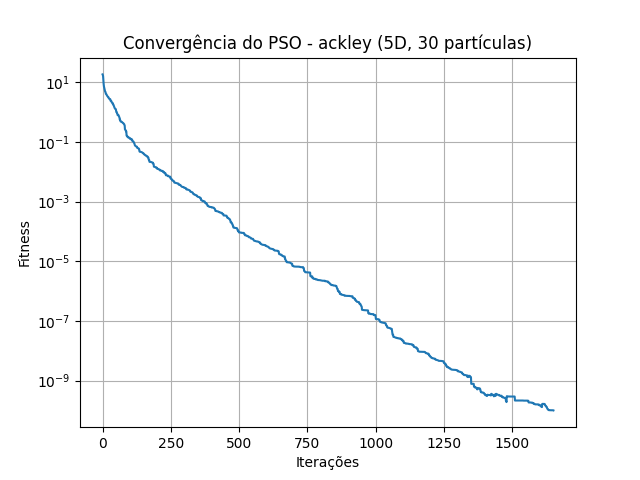
\includegraphics[width=.9\textwidth]{convergencia_ackley_5D.png}
  \caption{Convergência do PSO para Ackley (5 dimensões)}
  \label{fig:convergencia5d}
\end{figure}

\begin{figure}[H]
  \centering
  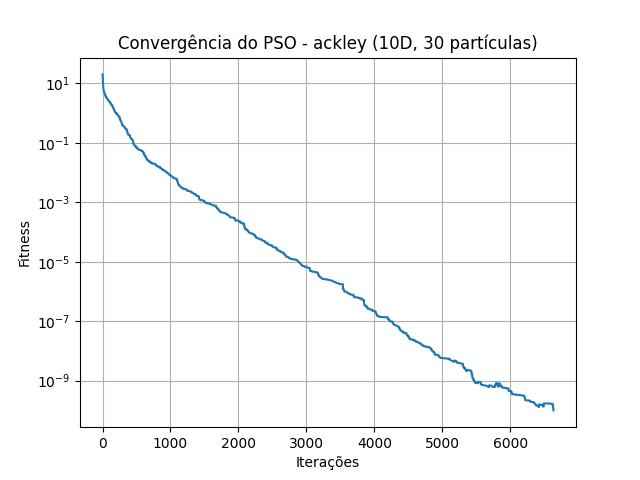
\includegraphics[width=.9\textwidth]{convergencia_ackley_10D.png}
  \caption{Convergência do PSO para Ackley (10 dimensões)}
  \label{fig:convergencia10d}
\end{figure}

Os resultados mostram que o PSO foi capaz de encontrar soluções próximas do ótimo global em ambas as dimensões, com convergência mais rápida para 5 dimensões.

\section{Análise dos resultados obtidos.}
\label{sec:analise_dos_resultados_obtidos}

A análise dos resultados evidencia que o PSO apresenta desempenho robusto na otimização das funções de Ackley e Griewank. Observa-se que, para menor dimensionalidade (5D), o algoritmo converge mais rapidamente e com menor variabilidade entre as execuções. Para 10 dimensões, a convergência é mais lenta e a variabilidade dos resultados aumenta, refletindo a maior complexidade do espaço de busca.

O ajuste dos parâmetros $c_1$ e $c_2$ mostrou-se adequado, promovendo um equilíbrio entre exploração e intensificação. O aumento do número de partículas ou de iterações pode contribuir para uma convergência ainda mais próxima do ótimo em instâncias de maior dimensão.

\section{Conclusões e Trabalhos Futuros}
\label{sec:conclusoes_e_trabalhos_futuros}

Neste trabalho, foi apresentada uma implementação do algoritmo \textbf{Particle Swarm Optimization} para otimização das funções de Ackley e Griewank. Os experimentos demonstraram a eficácia do PSO em encontrar soluções de alta qualidade, especialmente em espaços de menor dimensão.

Como trabalhos futuros, propõe-se a avaliação do PSO em outras funções de benchmark, a análise do impacto de diferentes estratégias de parametrização (como variação dinâmica dos coeficientes) e a comparação com outros algoritmos metaheurísticos, como Algoritmos Genéticos e Simulated Annealing.

Além disso, a aplicação do PSO em problemas reais de otimização, bem como o estudo de variantes do algoritmo (como PSO com topologias de vizinhança ou versões híbridas), constitui uma linha promissora para pesquisas futuras.

\bibliographystyle{sbc}
\bibliography{sbc-template}

\end{document}
